\documentclass{beamer}

\useoutertheme[glossy]{wuerzburg}
\useinnertheme[shadow,outline]{chamfered}
\usecolortheme{shark}
\beamertemplatenavigationsymbolsempty 

\usefonttheme{professionalfonts}
\let\digamma\relax
\usepackage[scale=0.85,stdmathitalics=true,romanfamily=casual]{lucimatx}
\usefonttheme[stillsansseriftext]{serif}


\usepackage{fancyvrb}

%% Fancy syntax coloring via pygments
\usepackage{minted}
\definecolor{bg}{rgb}{0.95,0.95,0.95}
\usemintedstyle{borland}


\newenvironment{Rcode}
{\VerbatimEnvironment
 \begin{minted}[fontsize=\scriptsize,baselinestretch=1]{r}}%
{\end{minted}}

\newenvironment{Pcode}
{\VerbatimEnvironment
 \begin{minted}[fontsize=\scriptsize,baselinestretch=1]{python}}%
{\end{minted}}

\newenvironment{Code}[1]
{\VerbatimEnvironment
 \begin{minted}[fontsize=\scriptsize,baselinestretch=1]{#1}}%
{\end{minted}}


\usepackage{textfit} % commands \scaletoheight{height}{text} and \scaletowidth{width}{text}

\usepackage{tikz}


\newtheorem{Alert}{Alert}
\newtheorem{Highlight}{Highlight}

\newcommand{\Species}[1]{{\rmfamily \itshape #1}}
\newcommand{\Real}{\ensuremath{\mathbb{R}}}
\newcommand{\RealN}{\ensuremath{\mathbb{R}^n}}
\newcommand{\RealP}{\ensuremath{\mathbb{R}^p}}
\newcommand{\Mtx}[1]{\ensuremath{\mathbf{#1}}}
\newcommand{\Inv}[1]{\ensuremath{#1^{-1}}}
\newcommand{\InvMtx}[1]{\ensuremath{\mathbf{#1}^{-1}}}
\newcommand{\Red}[1]{\textcolor{red}{#1}}
\newcommand{\PsInv}[1]{\ensuremath{\mathbf{#1}^{+}}}



\usepackage{pdfpages}

\parskip=0.5em

%===========================================================
\title{Scientific Computing for Biologists}
\subtitle{Lecture 8: (Dis)similarity and clustering}

\author{Instructor: Paul M. Magwene}
\date{01 November 2011}


\begin{document}

\begin{frame}
\titlepage
\end{frame}



%===========================================================
\begin{frame}
  \frametitle{Outline of Lecture}
  
\begin{itemize}
    \item Distance and dissimilarity measures
    \begin{itemize}
        \item Quantitative data
        \item Dichotomous data
        \item Qualitative data
    \end{itemize}
    \item Hierarchical clustering
    \item Neighbor-joining
    \item Multidimensional scaling (MDS)    
    \item Minimum Spanning Tree (MST)
\end{itemize}     
  
\end{frame}
%===========================================================

%===========================================================
\begin{frame}
  \frametitle{Similarity/Dissimilarity}

\begin{block}{Intuition}
Similarity is a measure of ``likeness'' between two entities of interest. Dissimilarity is the complement of similarity.
\end{block}


\begin{itemize}
\item Dissimilarities may be converted to similarities (and vise versa) by taking any monotonically decreasing function. For example:
\[
s = 1 - d_{ij}  \ \mbox{(for $0 \leq d_{ij} \leq 1$)}
\]
\item Dissimilarities are usually in range $0 \leq d_{ij} \leq C$ where $C$ is the maximum dissimilarity
\item Distances are one measure of dissimilarity but distances are unbounded to the right
\[
d_{ij} \in [0,\infty]
\]
\end{itemize}
\end{frame}
%===========================================================

%===========================================================
{ 
\setbeamercolor{background canvas}{bg=} 
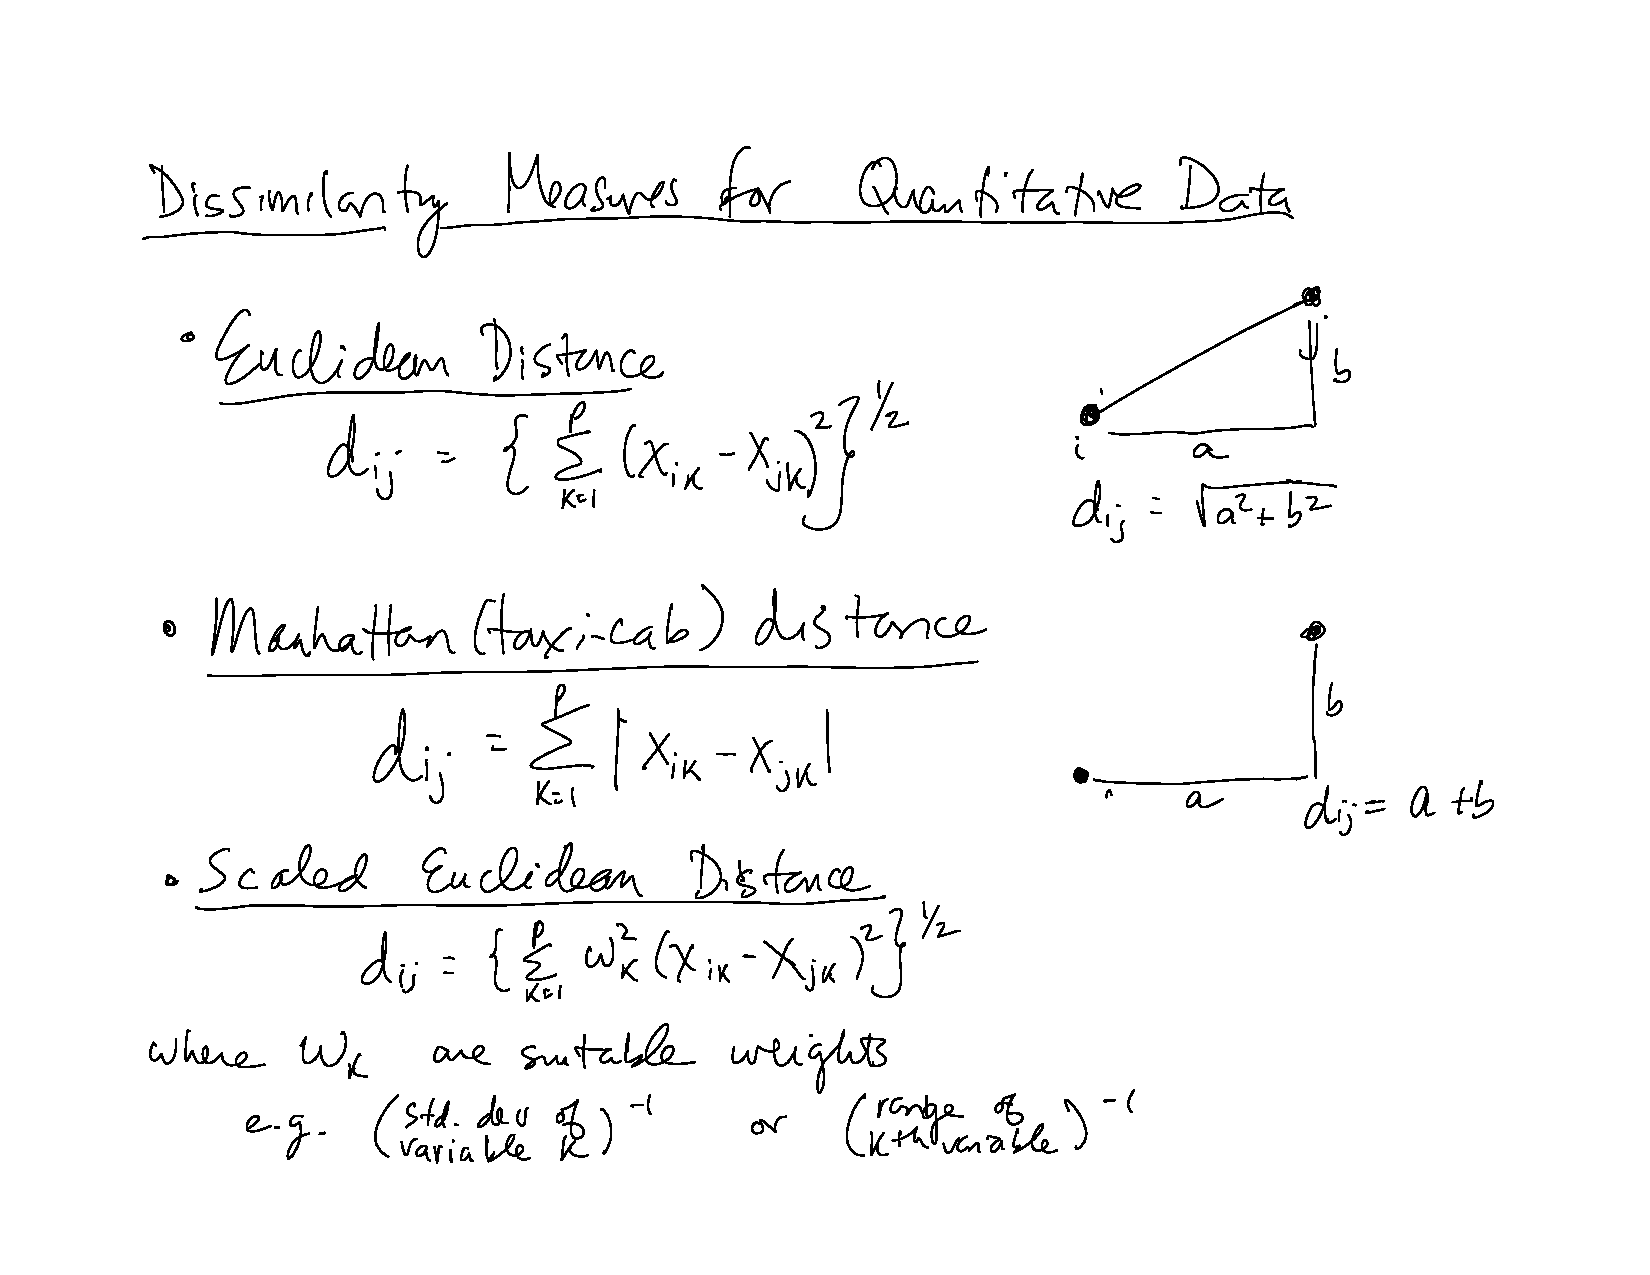
\includepdf[pages=1-16]{lecture7-clustering.pdf}
}
%===========================================================

%===========================================================
%% Neighbor-joining

\begin{frame}[shrink=5]
\frametitle{Neighbor Joining}

Originally described by Saitou and Nei, 1987.

\begin{block}{Goal}
Tries to create the (unrooted) tree topology with the least branch length
(minimum-evolution criterion).
\end{block}

Basic algorithm:
\begin{enumerate}
\item Calculate matrix $Q$ (next slide) from the distance matrix
\item Find the pair of taxa in $Q$ with the lowest value; create a node on the tree that joins these two taxa (i.e. the closest neighbors)
\item Calculate the distance of each of the taxa in the pair to this new node
\item Calculate the distance of all taxa outside of this pair to the new node
\item Repeat from step 1 using the distances calculated in the previous step
\end{enumerate}

\end{frame}
%===========================================================

%===========================================================
\begin{frame}
\frametitle{Neighbor Joining, cont.}

\[
Q_{ij} = (r - 2) d_{ij} - (R_i + R_j)
\]

where $r$ is the number of taxa, $d_{ij}$ is the distance between taxa $i$ and $j$ and $R_k$ is the row sum over row $k$ of the distance matrix ($R_k=\sum_i d_{ik}$).

\medskip

When nodes $i$ and $j$ are joined they are replaced by a node, $A$, with distance to a remaining node $k$ given by:
\[
d_{Ak} = \frac{1}{2} (d_{ik} + d_{jk} - d_{ij})
\]
    
\end{frame}
%===========================================================

%===========================================================
\begin{frame}
\frametitle{NJ example from Saitou and Nei 1987}
\begin{center}
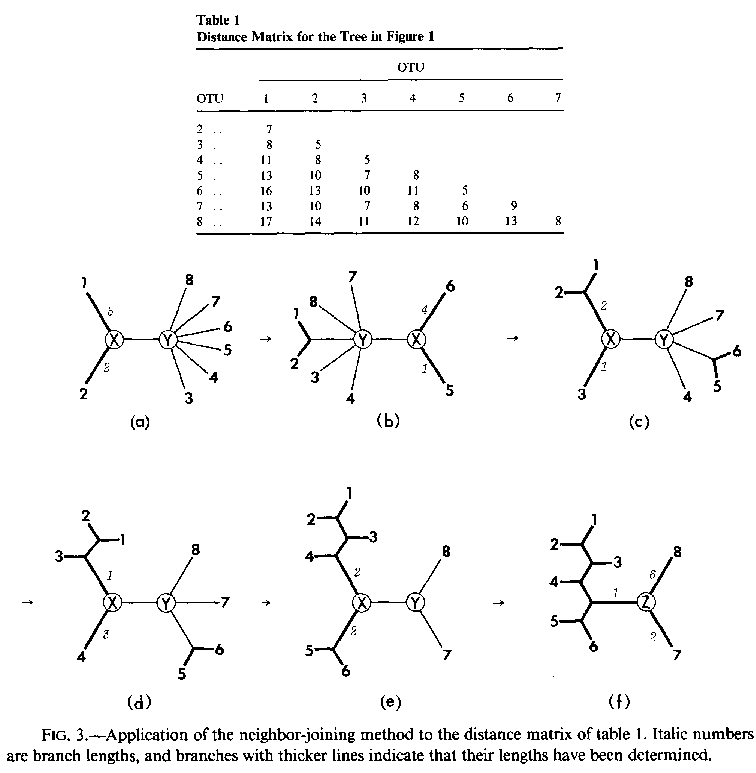
\includegraphics[height=3.2in]{saitou-nj-example.pdf}    
\end{center}
\end{frame}
%===========================================================




%===========================================================
\begin{frame}
  \frametitle{Multidimensional Scaling (MDS)}

\begin{block}{Goal}
Given dissimilarities between objects, $d_{ij}$, estimate a $k$-dimensional set of points, \Mtx{X}, such that $|x_i - x_j| \approx d_{ij}$.
\end{block}


\end{frame}
%===========================================================

%===========================================================
\begin{frame}[shrink=5]
\frametitle{Derivation of MDS}

\begin{block}{Motivation}
    If we know the coordinates of $n$ points in $p$-dimensional space, we can easily calculate the Euclidean distances between every pair of points. \alert{Can we reverse this process, starting with the distances and getting back the coordinates points?} 
\end{block}

Consider a data matrix \Mtx{X} ($n \times p$).  Let  $\Mtx{Q} = \Mtx{X}\Mtx{X}'$ be a $n \times n$ matrix, where
\[
q_{rs} = \sum_{j=1}^p x_{rj}x_{sj}
\]

If $d_{rs}^2$ is the squared Euclidean distance between points $r$ and $s$ then we can write this as:
\begin{eqnarray*}
d_{rs}^2 &=& \sum_{j=1}^p (x_{rj}-x_{sj})^2 \\
         &=& q_{rr} + q_{ss} - 2q_{rs}
\end{eqnarray*}

\end{frame}
%===========================================================

%===========================================================
\begin{frame}[shrink=5]
\frametitle{Derivation of MDS, cont.}

With a little bit of simple algebra we can show that:
\[
q_{rs} = -\frac{1}{2}(d_{rs}^2- d_{r.}^2 - d_{.s}^2 - d_{..}^2)
\]

where a dot represent the average of values over the corresponding suffix: $d_{r.}^2$ is the average over the $r$th row of matrix $\Mtx{D}=(d_{ij}^2)$, $d_{.s}^2$ is the average over the $s$th column of \Mtx{D}, and $d_{..}^2$ is the average of all elements of \Mtx{D}.So, given \Mtx{D}, the squared interpoint distances, we can regenerate \Mtx{Q}. 

Since \Mtx{Q} is symmetric, we can use eigendecomposition to write $\Mtx{Q}=\Mtx{T}\Mtx{\Lambda}\Mtx{T}'$  where $\Mtx{\Lambda}$ is a diagonal matrix of eigenvalues of \Mtx{Q} and \Mtx{T} is the matrix of eigenvectors. Furthermore we can write $\Mtx{Q}=\Mtx{T}\Mtx{\Lambda}\Mtx{T}'=\Mtx{T}\Mtx{\Lambda}^{\frac{1}{2}}\Mtx{\Lambda}^{\frac{1}{2}}\Mtx{T}'= \Mtx{X}\Mtx{X}'$ where $\Mtx{X}=\Mtx{T}\Mtx{\Lambda}^{\frac{1}{2}}$. 

\alert{Thus we've found how to get \Mtx{X} from the squared distances.}

{\footnotesize See Krzanowski, W.\ J. (2000) Principles of multivariate analysis, for full details.}
\end{frame}
%===========================================================

%===========================================================
\begin{frame}
\frametitle{Algorithm for MDS}

Given an $n \times n$ matrix of dissimilarities, $\Mtx{D}$, with elements $d_{ij}$:

\begin{enumerate}
\item Form matrix, $\Mtx{E}$, where $e_{ij} = -\frac{1}{2} d_{ij}^2$

\item Subtract from each element of $\Mtx{E}$ the means of the row and column in which it is located and the mean of all elements of $\Mtx{E}$; call the resulting matrix $\Mtx{F}$

\item Calculate the eigenvalues ($\lambda_i$) and eigenvectors $\Mtx{v}_i$ of $\Mtx{F}$, sorted in decreasing order. Eigenvectors should be normalized (i.e. $\Mtx{v}_i \cdot \Mtx{v}_i = 1$).

\item The coordinates of the $n$ point on the $j$-th axis are given $\sqrt{\lambda_j}\Mtx{v}_j$

\end{enumerate}

\end{frame}
%===========================================================

%===========================================================
\begin{frame}
  \frametitle{Potential MDS Complications}

If the $d_{ij}$ are metric (i.e. $d_{ij} \leq d_{ik} + d_{kj}$) than $\Mtx{F}$ is always positive semidefinite (psd; i.e. eigenvalues $\geq 0$).

\medskip
If $\Mtx{F}$ is not psd than how do you handle negative eigenvalues?

\begin{itemize}

\item Most common approach is only to consider positive eigenvalues
\item This is OK if negative eigenvalues have small magnitude
\item If negative eigenvalues are large than approximation tends to be poor

\end{itemize}


\end{frame}
%===========================================================

%===========================================================
\begin{frame}
  \frametitle{Multidimensional Scaling: Keep in mind...}

\begin{itemize}
\item The configuration produced by any MDS method is indeterminate with respect to translation, rotation, and reflection.

\end{itemize}


\end{frame}
%===========================================================

%===========================================================
\begin{frame}
  \frametitle{Relationship between metric MDS and PCA}
  
 If the $d_{ij}$ are Euclidean distances from a data matrix, $\Mtx{X}$, then metric MDS of $\Mtx{D}$ yields the PC scores obtained by PCA of $\Mtx{X}$.
 
 \medskip
  \begin{block}{Interpretation}
PCA and MDS are dual methods:
\begin{itemize}
  \item One operates on variable space (PCA)
  \item The other operates on subject space (MDS)
\end{itemize}
\end{block}

\end{frame}
%===========================================================

%===========================================================
\begin{frame}
  \frametitle{Other Metric MDS Approaches}
  
\begin{itemize}
\item Classical MDS minimizes:
\[
\sum_i \sum_j(\delta_{ij}^2 - d_{ij}^2)
\]

where $\delta_{ij}$ is the distance between observations $i$ and $j$ in the MDS approximation.

\item Alternates approaches try to minimize other measures of discrepancy. For example, ``Sammon MDS" minimizes:
\[
\sum_i \sum_j (\delta_{ij} - d_{ij})^2
\]
\end{itemize}
\end{frame}
%===========================================================

%===========================================================
\begin{frame}
  \frametitle{Non-Metric MDS}

Non-metric MDS approaches try to preserve only the rank order of the distances.

If
\[
d_{i1,j1} < d_{i2,j2} < \cdots< d_{im,jm}
\]

then
\[
\delta_{i1,j1} < \delta_{i2,j2} < \cdots< \delta_{im,jm}
\]

Shepard-Kruskal solution:

\begin{itemize}
\item Find $\hat{d}_{ij}$ that minimizes:
\[
\mbox{STRESS} = \sqrt{ \{ \frac{\sum \sum_{i < j}(d_{ij}-\hat{d}_{ij})^2 }{\sum \sum d_{ij}^2} \} }
\]
\end{itemize}
  
\bigskip

\end{frame}
%===========================================================

%===========================================================
\begin{frame}
  \frametitle{MDS Example: Road Distances}

Input $\Mtx{D}$: road distances between U.S. cities

\begin{center}
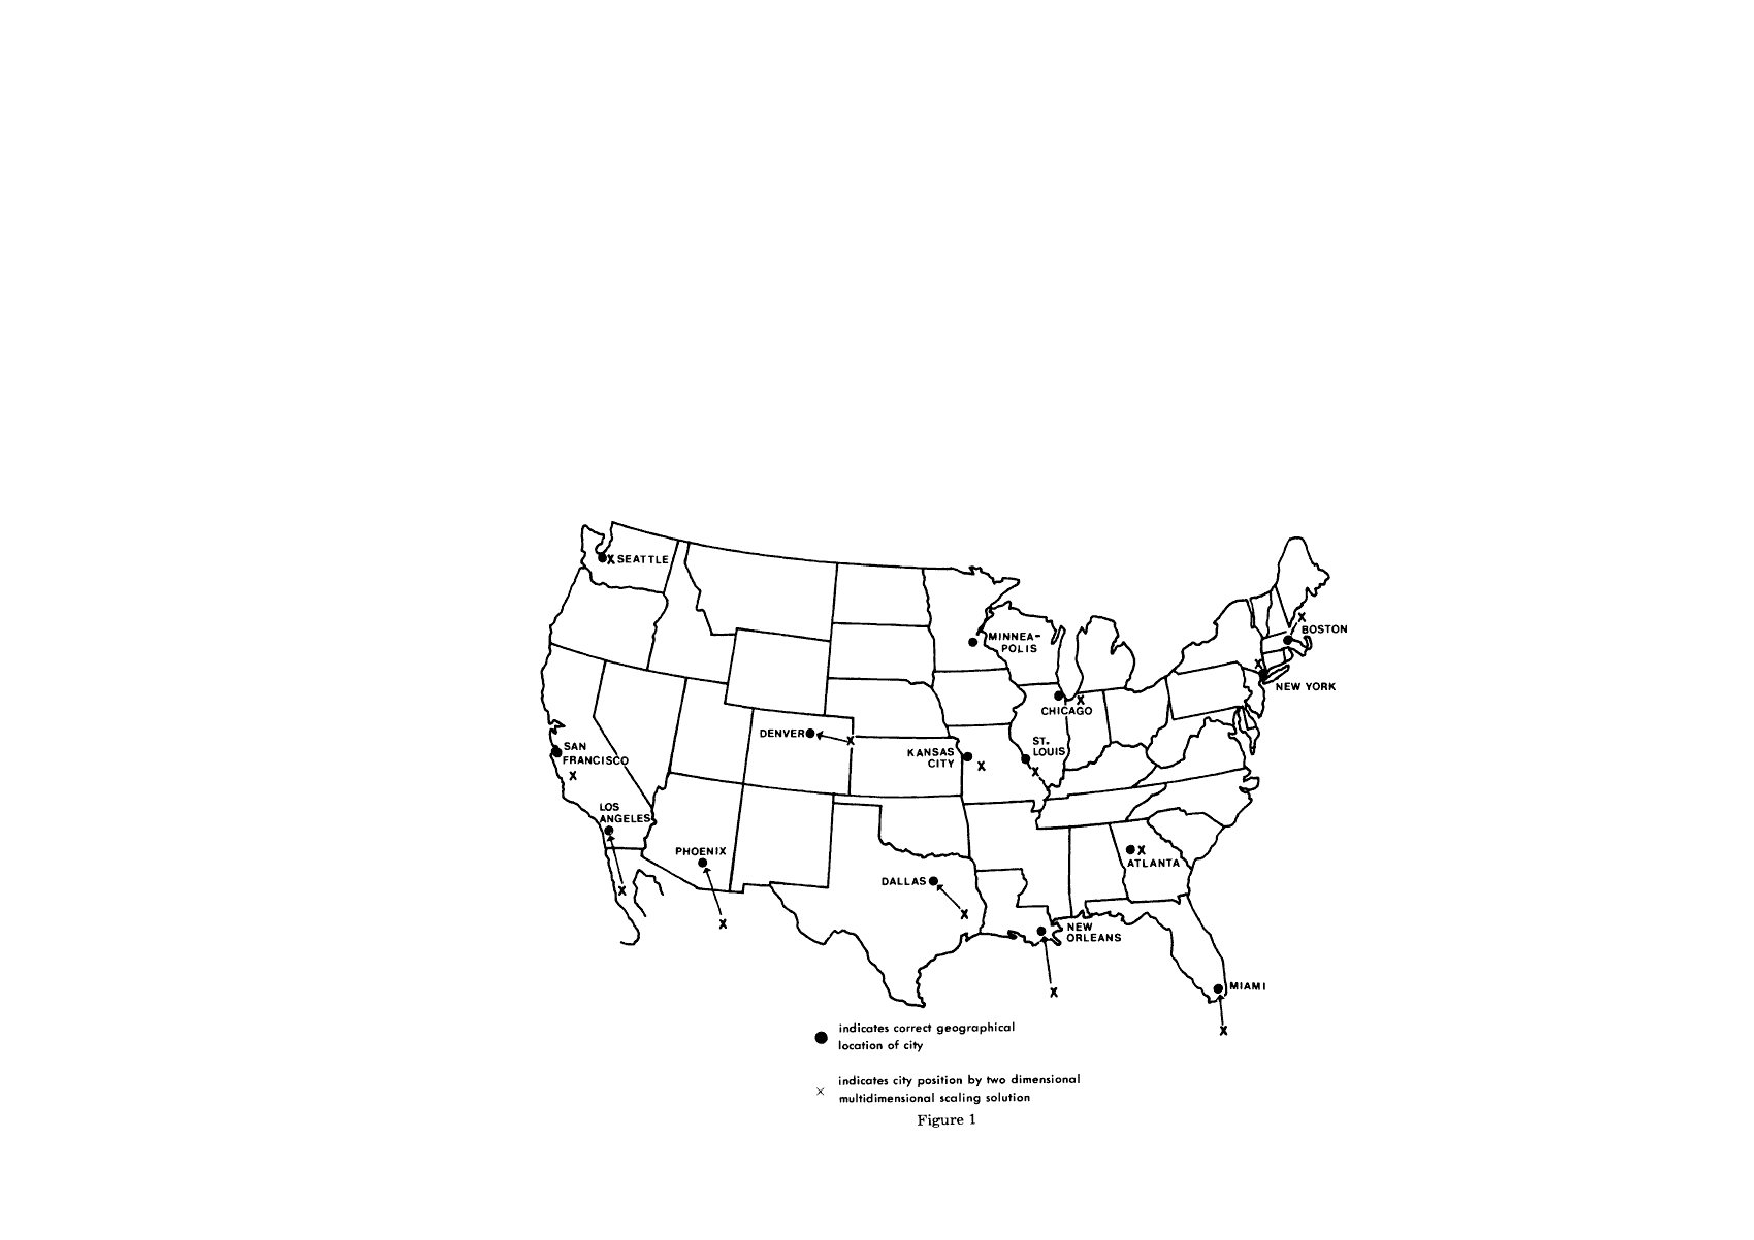
\includegraphics[height=2.9in]{mds-road}
\end{center}

\end{frame}
%===========================================================

%===========================================================
\begin{frame}
  \frametitle{More MDS Examples I}
  
{\footnotesize
\textbf{Source}: Zhivotovsky et al. (2003). Features of evolution and expansion of modern humans, inferred from genomwide microsatellite markers. Am J Hum Genet 72: 1171�1186.

\textbf{Dissimilarities}: $F_{ST}$'s between population samples.
}

\begin{center}
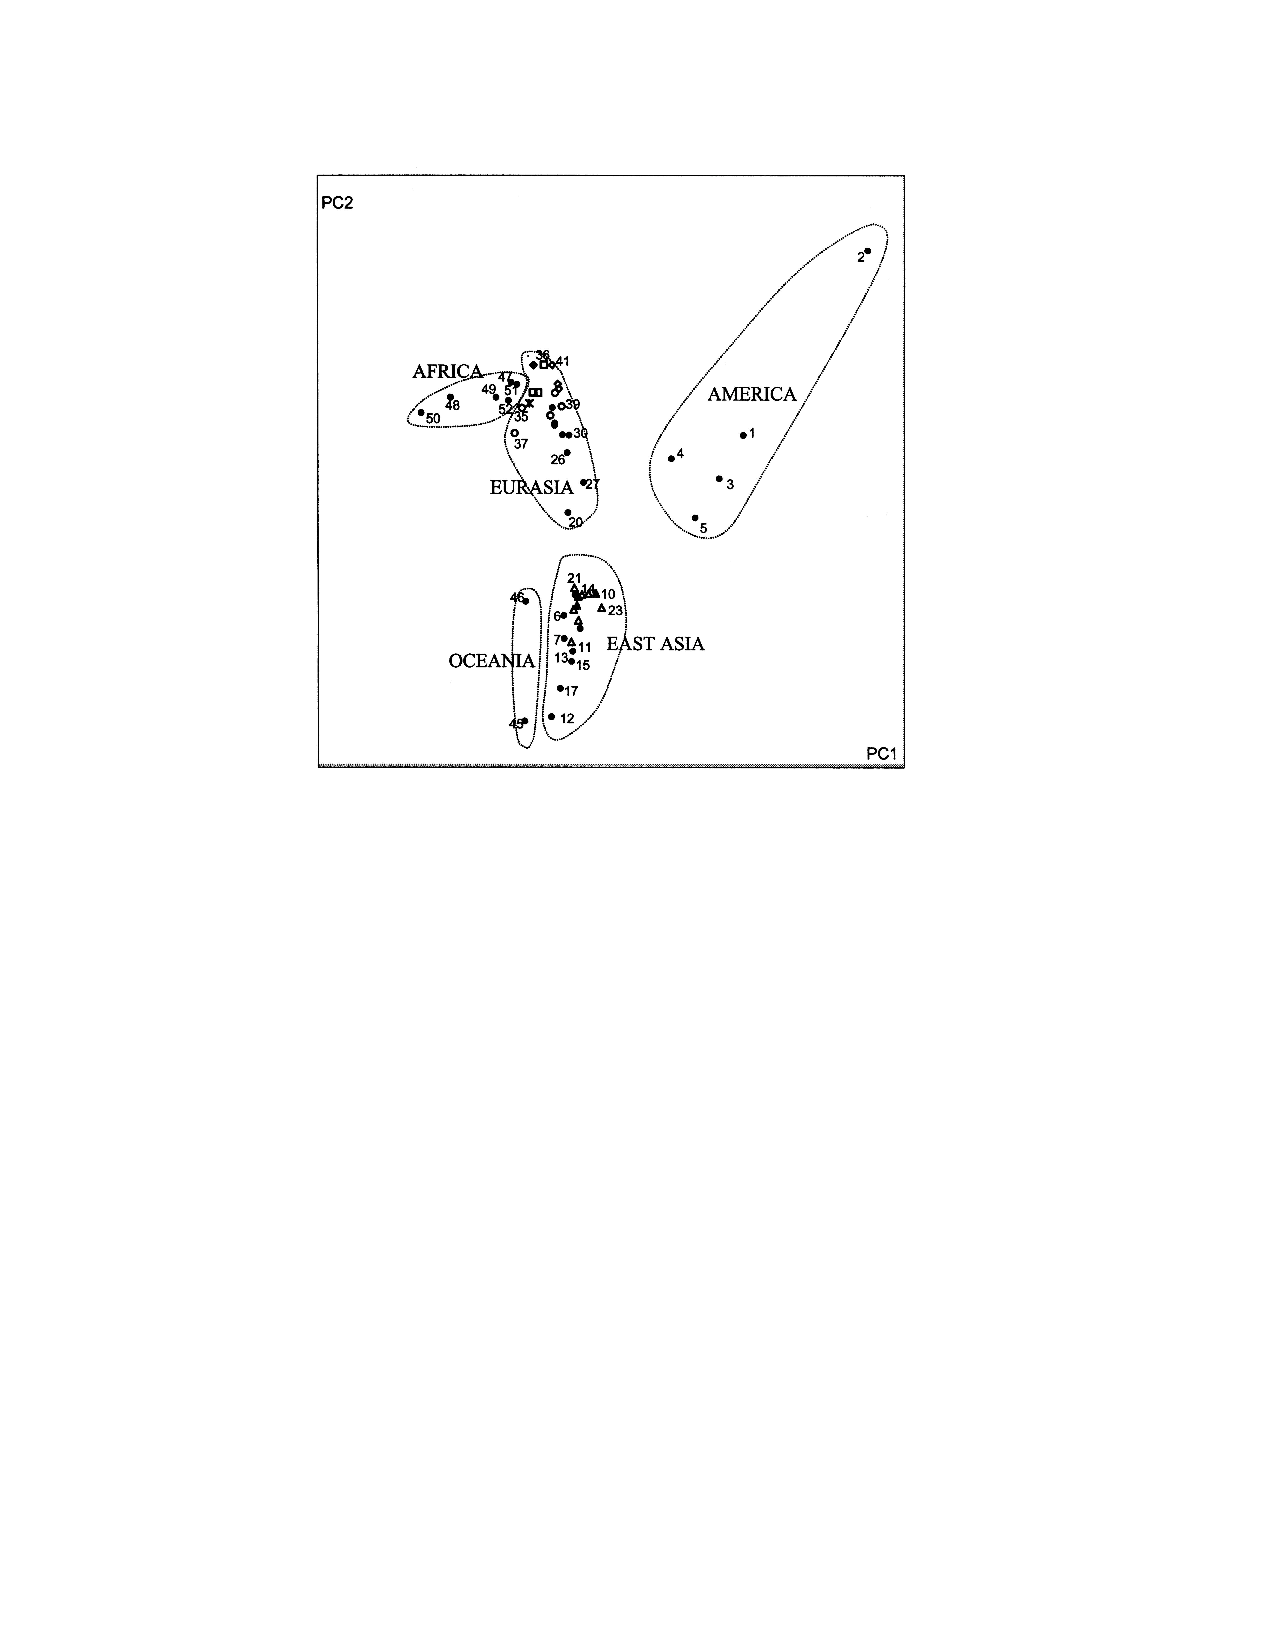
\includegraphics[height=2.25in]{zhivotsky-etal-figure}
\end{center}

\end{frame}
%===========================================================

%===========================================================


\begin{frame}
  \frametitle{Good MDS References}
  
Kenkel, N. C. and L. Oroloci (1986). Applying metric and nonmetric multidimensional scaling to ecological studies: Some new results. Ecology 67:919-928


\end{frame}
%===========================================================


%===========================================================
\begin{frame}
  \frametitle{Minimum Spanning Tree}

\begin{block}{Goal}
Construct a tree that connects all points in the data set and whose total length is minimized.
\end{block}

\emph{Statistical applications}
\begin{itemize}
    \item highlights close neighbors in a data set
    \item useful check for distortions produced by projection techniques
    \item tests of normality
\end{itemize}
\medskip

\emph{Other applications}
\begin{itemize}
    \item urban planning/engineering
    \item circuit design
\end{itemize}

\end{frame}
%===========================================================

%===========================================================
\begin{frame}
  \frametitle{Example Data Set}

\begin{center}
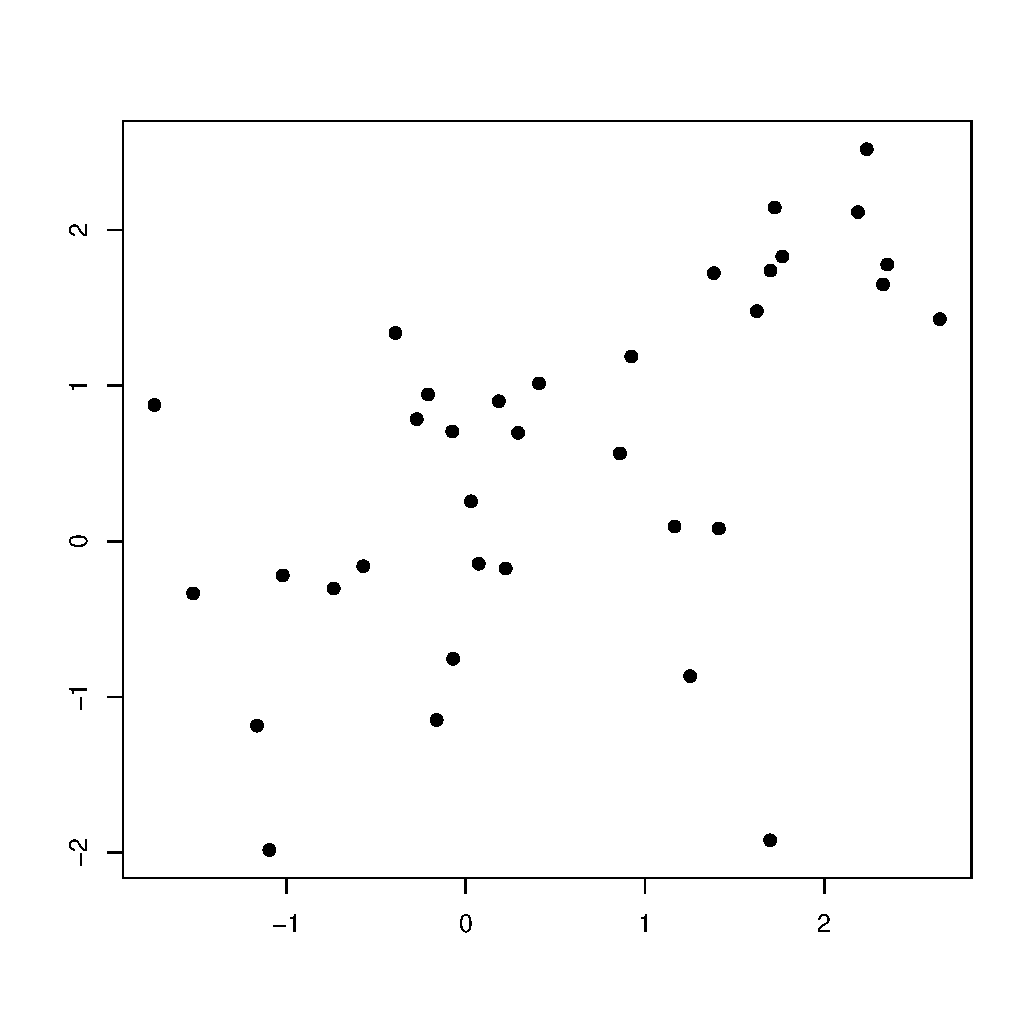
\includegraphics[height=3.1in]{points-only}
\end{center}
\end{frame}
%===========================================================

%===========================================================
\begin{frame}
  \frametitle{Minimum Spanning Tree: Example}

  
\begin{center}
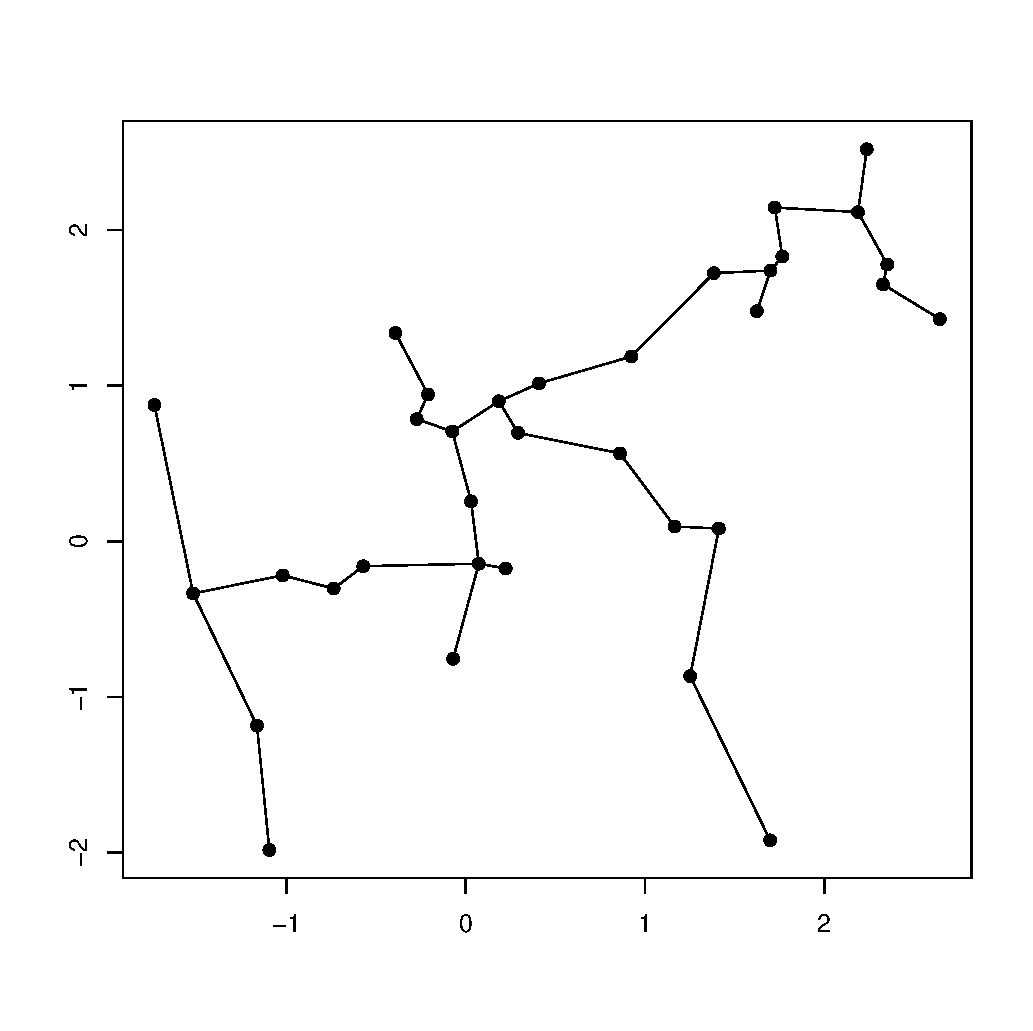
\includegraphics[height=3.1in]{points-mst}
\end{center}
\end{frame}
%===========================================================

%===========================================================
\begin{frame}
  \frametitle{Relationship between MST and Single Linkage Clustering}


\begin{itemize}

\item Cut a single linkage dendrogram at height, $\delta \dashrightarrow$ clusters

\item Remove all edges in the MST with length $\geq \delta \dashrightarrow$ subgraphs corresponding to the same clusters

\end{itemize}

\end{frame}
%===========================================================

%===========================================================
\begin{frame}
  \frametitle{A Generic MST Algorithm}


\textbf{Input}: dissimilarity matrix, \Mtx{D}, between each object (point) of interest
\begin{enumerate}
\item Create a graph, G, where  $V = \{v_1,\ldots,v_n\}$ and $E =\{\}$ ($E$ initially empty)
\item Find the smallest dissimilarity, $d_{ij}$ where (i,j) is not in $E$.
\item Add (i,j) to $E$ if (i,j) does not create a cycle
\item Repeat from step 2 until every vertex is included in at least one edge
\end{enumerate}

Not particularly efficient algorithm, but simple. More efficient algorithms for finding MSTs include Kruskal's Algorithm and Prim's algorithm.

\end{frame}
%===========================================================

%===========================================================
\begin{frame}
  \frametitle{Applications of the MST}

MST tends to highlight close neighbors; can be used to look for distortions associated with projections to lower dimensional spaces.

\begin{block}{Using the MST to look for Projection Distortion}
\begin{itemize}
    \item  Calculate the MST based on dissimilarity in a high-dimensional space
    \item Draw the MST edges among points in the projection space (e.g. MDS or PCA)
    \item MST edges that cross highlight geometric relationships among points that are not well represented by the projection
\end{itemize}
\end{block}
\end{frame}
%===========================================================



\end{document}



%===========================================================
\begin{frame}
  \frametitle{XXX}

\end{frame}
%===========================================================

